\documentclass[11pt]{article}

\usepackage{fullpage}
\usepackage{graphicx}
\usepackage{amsmath}
\usepackage{amssymb}
\usepackage{amsthm}
\usepackage{fancyvrb}

\parindent0in
\pagestyle{plain}
\thispagestyle{plain}

\newcommand{\myname}{Mehshan Mustafa}
\newcommand{\dated}{\today}

\newenvironment{theorem}[2][Theorem]{\begin{trivlist}
\item[\hskip \labelsep {\bfseries #1}\hskip \labelsep {\bfseries #2.}]}{\end{trivlist}}
\newenvironment{lemma}[2][Lemma]{\begin{trivlist}
\item[\hskip \labelsep {\bfseries #1}\hskip \labelsep {\bfseries #2.}]}{\end{trivlist}}
\newenvironment{exercise}[2][Exercise]{\begin{trivlist}
\item[\hskip \labelsep {\bfseries #1}\hskip \labelsep {\bfseries #2.}]}{\end{trivlist}}
\newenvironment{problem}[2][Problem]{\begin{trivlist}
\item[\hskip \labelsep {\bfseries #1}\hskip \labelsep {\bfseries #2.}]}{\end{trivlist}}
\newenvironment{question}[2][Question]{\begin{trivlist}
\item[\hskip \labelsep {\bfseries #1}\hskip \labelsep {\bfseries #2.}]}{\end{trivlist}}
\newenvironment{corollary}[2][Corollary]{\begin{trivlist}
\item[\hskip \labelsep {\bfseries #1}\hskip \labelsep {\bfseries #2.}]}{\end{trivlist}}
\newenvironment{solution}{\begin{proof}[Solution]}{\end{proof}}
\newenvironment{idea}[2][Proof Idea.]{\textit{#1} #2}

\begin{document}
\textbf{Introduction to the Theory of
Computation}\hfill\textbf{\myname}\\[0.01in]
\textbf{Chapter 1: Reqular Languages}\hfill\textbf{\dated}\\
\smallskip\hrule\bigskip

\begin{problem}{1.43}
Let A be any language. Define $DROP-OUT(A)$ to be the language containing all strings that can be obtained by removing one symbol from a string in A. Thus, $DROP-OUT (A) = \{xz \ | \ xyz \in A \ where \ x, \ z \in \Sigma^{*}, \ y \in \Sigma\}$. Show that the class of regular languages is closed under the $DROP-OUT$ operation. Give both a proof by picture and a more formal proof by construction as in Theorem 1.47.
\end{problem}

\begin{problem}[Part]{1}
Proof by picture. Let $\Sigma=\{a,b\}$ and $A=\{w \ | \ w \ has \ odd \ length\}$. $A$ contains the strings $a$, $b$, $aaa$, $aab$, and $bbb$. $DROP-OUT(A)$ contains all strings of even length, such as $\epsilon$, $aa$, $ab$, and $bb$.
\end{problem}

\begin{center}
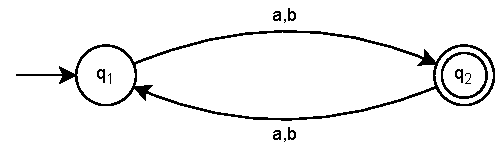
\includegraphics[scale=1]{Figures/Problem1.43a.pdf} \\
 The above DFA recognizes $A$.
\end{center}

The idea is to construct a finite automaton using the DFA of $A$, which drops one symbol at a time in strings of $A$. Take the DFA that recognizes $A$, for each state, keep all of its transitions, but also skip all transitions to the next states by adding $\epsilon$-transitions, because each symbol is represented by a tranistion in automata. After skipping a symbol, we need to make sure that no subsequent symbols are skipped. This can be achieved by using two copies of $A$'s DFA in the new finite automaton. One DFA selects a position to drop a symbol, while the other continues normally after that. The two DFAs are connected using $\epsilon$-transitions that simulate dropping of a symbol.
\begin{center}
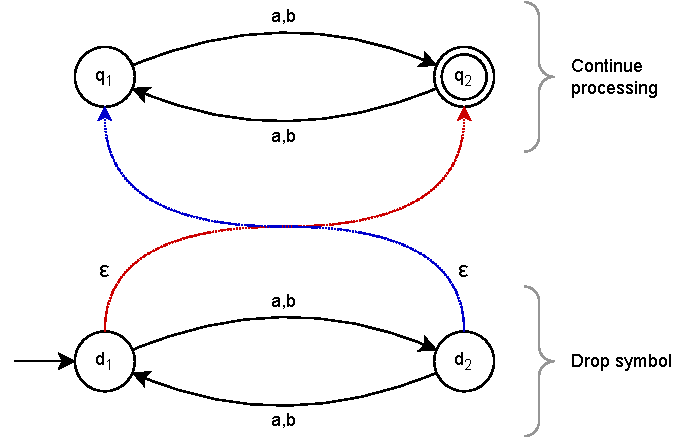
\includegraphics[scale=1]{Figures/Problem1.43b.pdf} \\
NFA that recognizes $DROP-OUT(A)$.
\end{center}

% TODO

% \begin{problem}[Part]{2}
% Formal proof by construction.
% \end{problem}

% \begin{proof}
% \end{proof}
\end{document}